\documentclass[11pt]{report}
\usepackage[utf8]{inputenc}
\usepackage[T1]{fontenc}
\usepackage{geometry}
\geometry{a4paper, margin=1in}
\usepackage{tikz}
\usetikzlibrary{shapes.geometric, arrows.meta, positioning, calc, fit, backgrounds}
\usepackage{makecell}
\usepackage{graphicx}
\usepackage{hyperref}

\tikzset{
    box/.style = {draw, rectangle, rounded corners, minimum width=2.5cm, minimum height=1cm, text centered, align=center, fill=white},
    db/.style = {draw, cylinder, shape border rotate=90, aspect=0.25, minimum height=1.5cm, minimum width=2.5cm, text centered, align=center, fill=white},
    diamondbox/.style = {draw, diamond, aspect=2, text centered, align=center, fill=white},
    arrow/.style = {-{Stealth[scale=1.2]}, thick},
    darrow/.style = {dashed, -{Stealth[scale=1.2]}},
    subgraph/.style = {draw, rectangle, rounded corners, dashed, inner sep=15pt, fill=gray!5}
}

\begin{document}

\chapter*{EchoScribe v2.0 Architecture Diagrams}

\section*{1. System Overview}
\resizebox{\textwidth}{!}{%
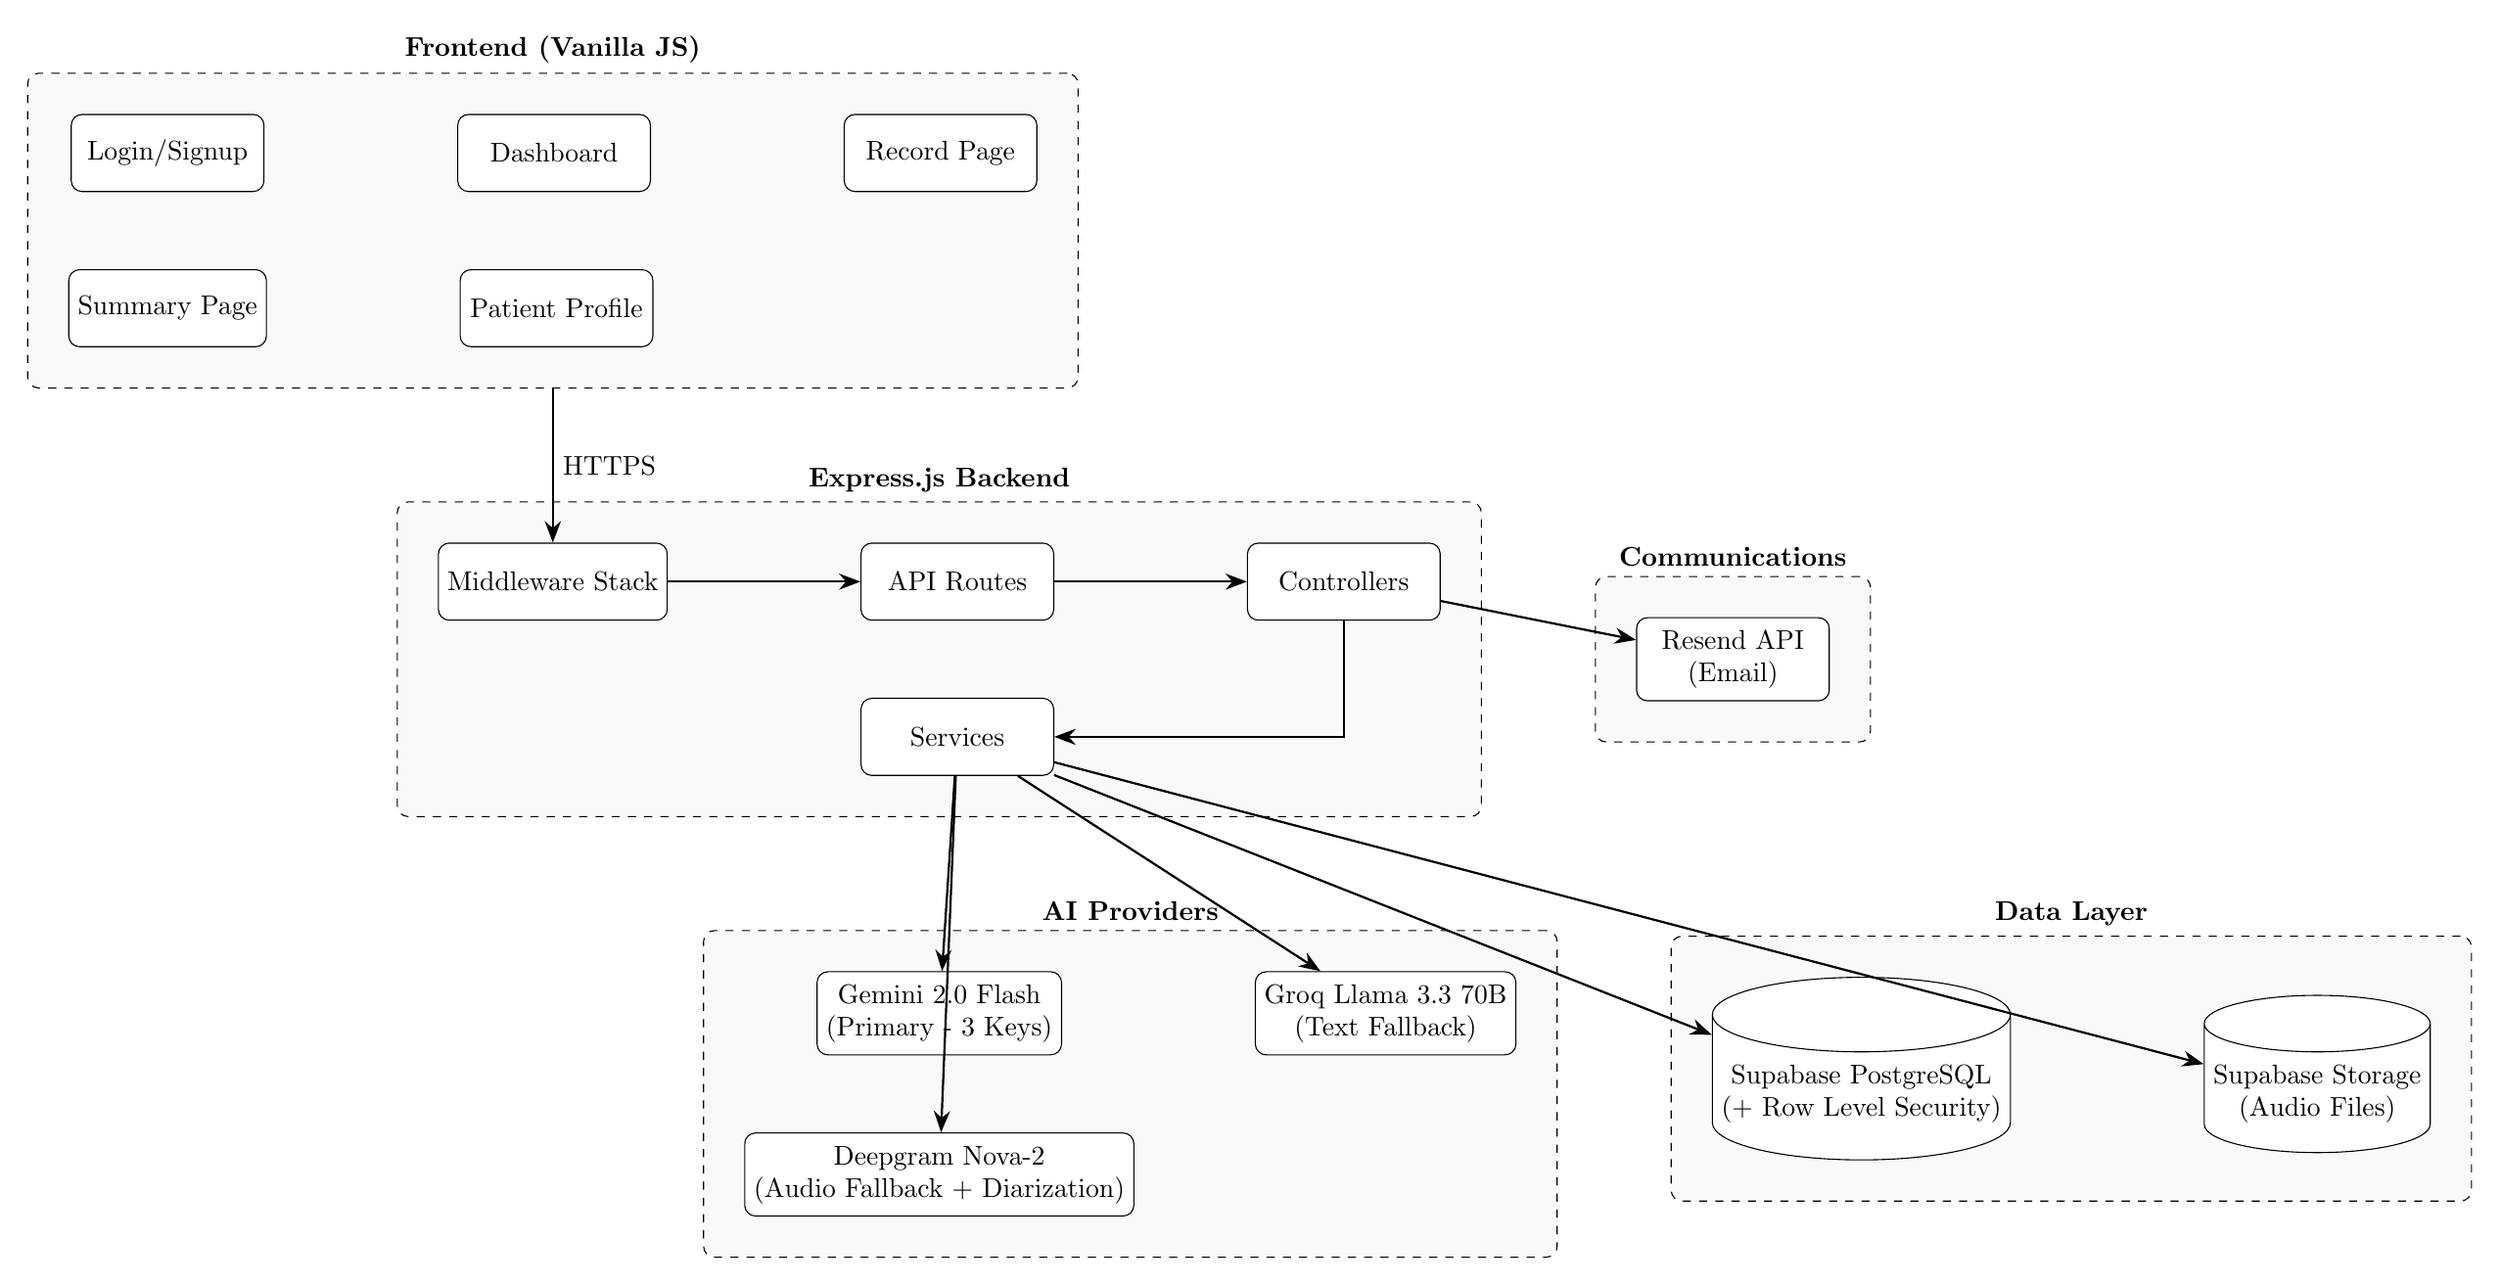
\begin{tikzpicture}[node distance=2cm and 2.5cm, >={Stealth[scale=1.2]}]

    % Frontend subgraph
    \node[box] (L) {Login/Signup};
    \node[box, right=of L] (D) {Dashboard};
    \node[box, right=of D] (R) {Record Page};
    \node[box, below=1cm of L] (S) {Summary Page};
    \node[box, right=of S] (P) {Patient Profile};
    \begin{scope}[on background layer]
        \node[subgraph, fit=(L)(D)(R)(S)(P), label=above:\textbf{Frontend (Vanilla JS)}] (Client) {};
    \end{scope}

    % Backend subgraph
    \node[box, below=2cm of Client] (MW) {Middleware Stack};
    \node[box, right=of MW] (RT) {API Routes};
    \node[box, right=of RT] (CT) {Controllers};
    \node[box, below=1cm of RT] (SV) {Services};
    \begin{scope}[on background layer]
        \node[subgraph, fit=(MW)(RT)(CT)(SV), label=above:\textbf{Express.js Backend}] (Server) {};
    \end{scope}

    % AI Providers subgraph
    \node[box, below=2cm of Server] (G) {\makecell{Gemini 2.0 Flash\\(Primary - 3 Keys)}};
    \node[box, right=of G] (GR) {\makecell{Groq Llama 3.3 70B\\(Text Fallback)}};
    \node[box, below=1cm of G] (DG) {\makecell{Deepgram Nova-2\\(Audio Fallback + Diarization)}};
    \begin{scope}[on background layer]
        \node[subgraph, fit=(G)(GR)(DG), label=above:\textbf{AI Providers}] (AI) {};
    \end{scope}

    % Database subgraph
    \node[db, right=2cm of AI] (SB) {\makecell{Supabase PostgreSQL\\(+ Row Level Security)}};
    \node[db, right=of SB] (ST) {\makecell{Supabase Storage\\(Audio Files)}};
    \begin{scope}[on background layer]
        \node[subgraph, fit=(SB)(ST), label=above:\textbf{Data Layer}] (Storage) {};
    \end{scope}

    % Comm subgraph
    \node[box, right=2cm of Server] (RS) {\makecell{Resend API\\(Email)}};
    \begin{scope}[on background layer]
        \node[subgraph, fit=(RS), label=above:\textbf{Communications}] (Email) {};
    \end{scope}

    % Edges
    \draw[arrow] (Client.south) -- node[right] {HTTPS} (MW.north);
    \draw[arrow] (MW) -- (RT);
    \draw[arrow] (RT) -- (CT);
    \draw[arrow] (CT) |- (SV);
    \draw[arrow] (CT) -- (RS);
    \draw[arrow] (SV) -- (G);
    \draw[arrow] (SV) -- (GR);
    \draw[arrow] (SV) -- (DG);
    \draw[arrow] (SV) -- (SB);
    \draw[arrow] (SV) -- (ST);

\end{tikzpicture}%
}
\end{center}

\newpage
\section*{2. AI Multi-Provider Failover Architecture}
\resizebox{\textwidth}{!}{%
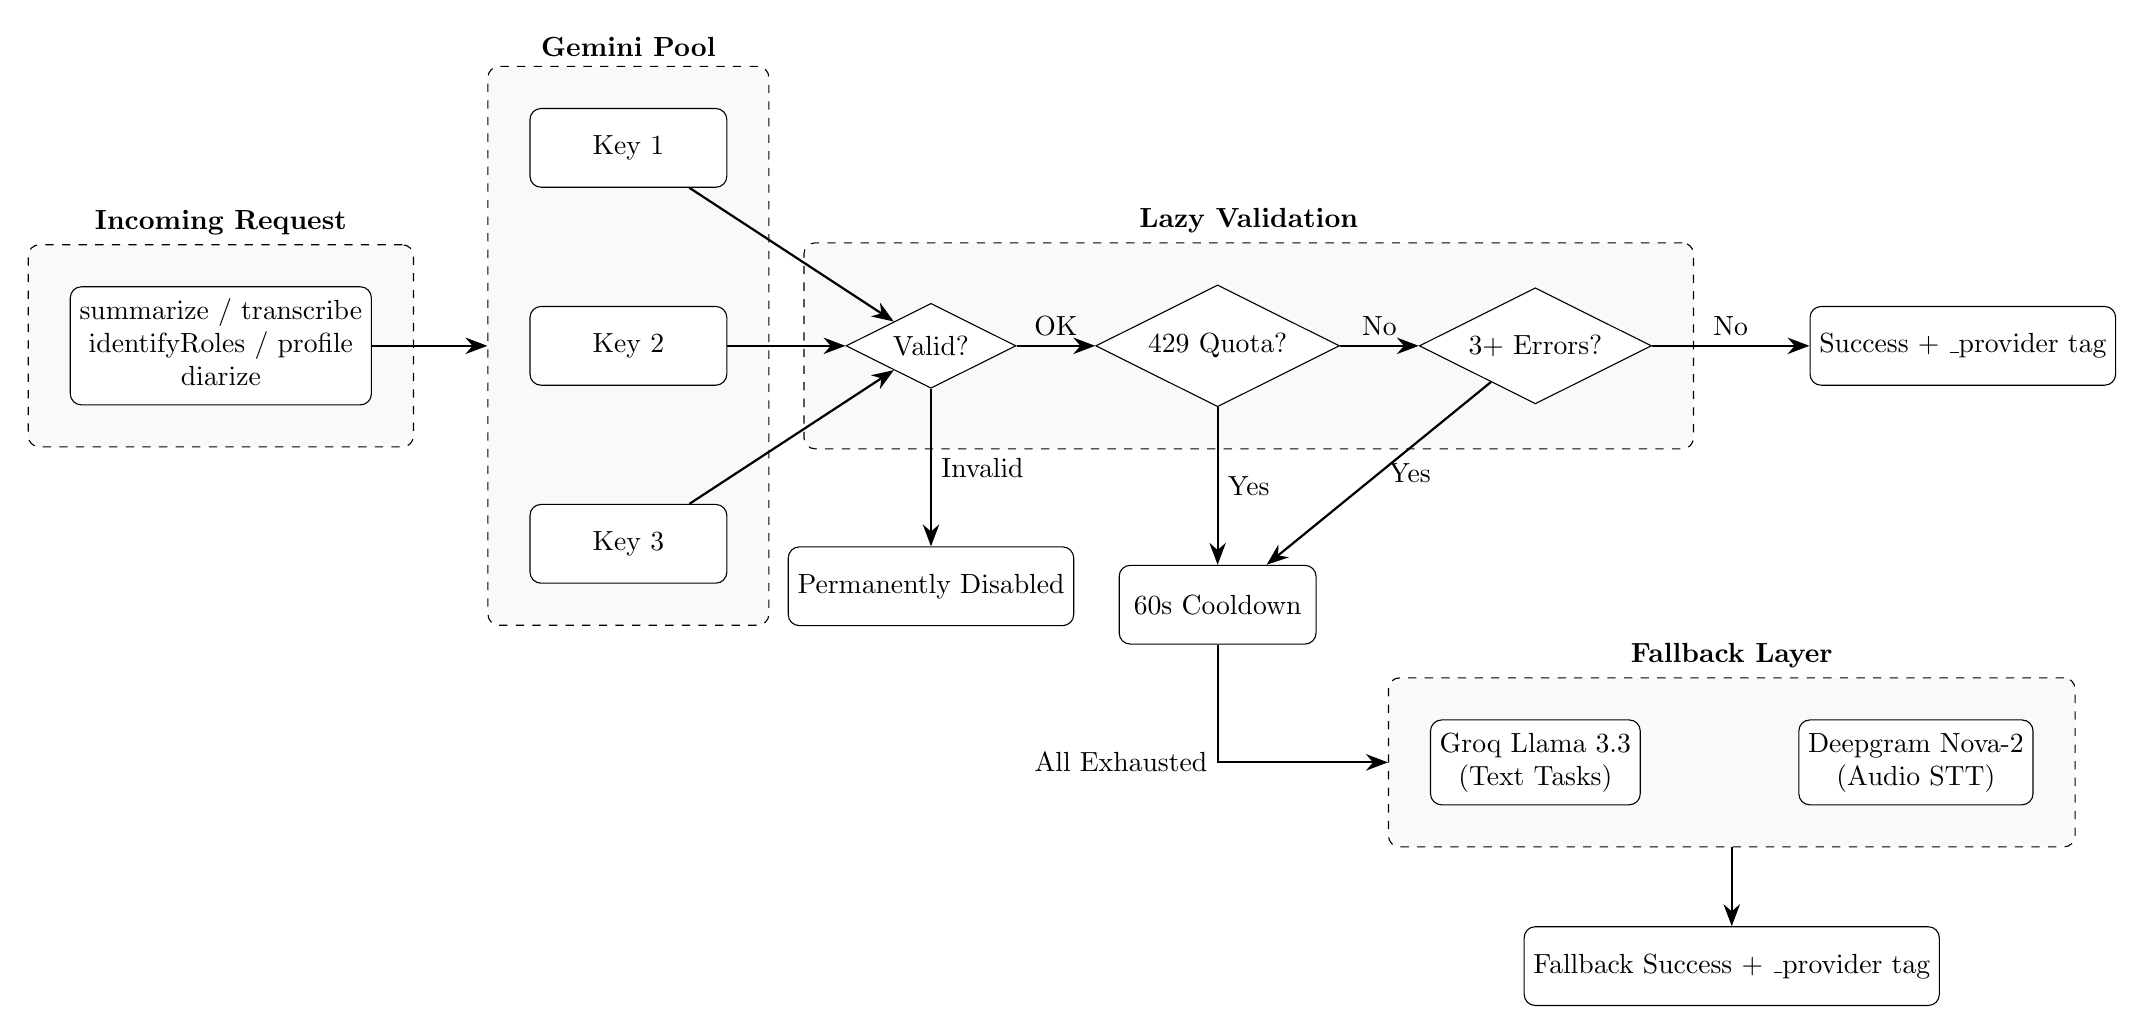
\begin{tikzpicture}[node distance=1.5cm and 2cm]
    \node[box] (REQ) {\makecell{summarize / transcribe\\identifyRoles / profile\\diarize}};
    \begin{scope}[on background layer]
        \node[subgraph, fit=(REQ), label=above:\textbf{Incoming Request}] (RequestLayer) {};
    \end{scope}

    \node[box, right=2cm of REQ] (K2) {Key 2};
    \node[box, above=of K2] (K1) {Key 1};
    \node[box, below=of K2] (K3) {Key 3};
    \begin{scope}[on background layer]
        \node[subgraph, fit=(K1)(K2)(K3), label=above:\textbf{Gemini Pool}] (Pool) {};
    \end{scope}

    \node[diamondbox, right=1.5cm of K2] (V1) {Valid?};
    \node[diamondbox, right=1cm of V1] (V2) {429 Quota?};
    \node[diamondbox, right=1cm of V2] (V3) {3+ Errors?};
    \begin{scope}[on background layer]
        \node[subgraph, fit=(V1)(V2)(V3), label=above:\textbf{Lazy Validation}] (Validation) {};
    \end{scope}

    \node[box, below=2cm of V1] (X) {Permanently Disabled};
    \node[box, below=2cm of V2] (CD) {60s Cooldown};
    \node[box, right=2cm of V3] (OK) {Success + \_provider tag};

    \node[box, below=4cm of V3] (GR) {\makecell{Groq Llama 3.3\\(Text Tasks)}};
    \node[box, right=of GR] (DG) {\makecell{Deepgram Nova-2\\(Audio STT)}};
    \begin{scope}[on background layer]
        \node[subgraph, fit=(GR)(DG), label=above:\textbf{Fallback Layer}] (Fallback) {};
    \end{scope}
    
    \node[box, below=1cm of Fallback] (OK2) {Fallback Success + \_provider tag};

    % Edges
    \draw[arrow] (REQ) -- (Pool.west);
    \draw[arrow] (K1) -- (V1);
    \draw[arrow] (K2) -- (V1);
    \draw[arrow] (K3) -- (V1);
    \draw[arrow] (V1) -- node[right] {Invalid} (X);
    \draw[arrow] (V1) -- node[above] {OK} (V2);
    \draw[arrow] (V2) -- node[right] {Yes} (CD);
    \draw[arrow] (V2) -- node[above] {No} (V3);
    \draw[arrow] (V3) -- node[right] {Yes} (CD);
    \draw[arrow] (V3) -- node[above] {No} (OK);
    \draw[arrow] (CD) |- node[left] {All Exhausted} (Fallback.west);
    \draw[arrow] (Fallback.south) -- (OK2);
\end{tikzpicture}%
}
\end{center}

\newpage
\section*{3. Request Flow (Middleware Pipeline)}
\resizebox{\textwidth}{!}{%
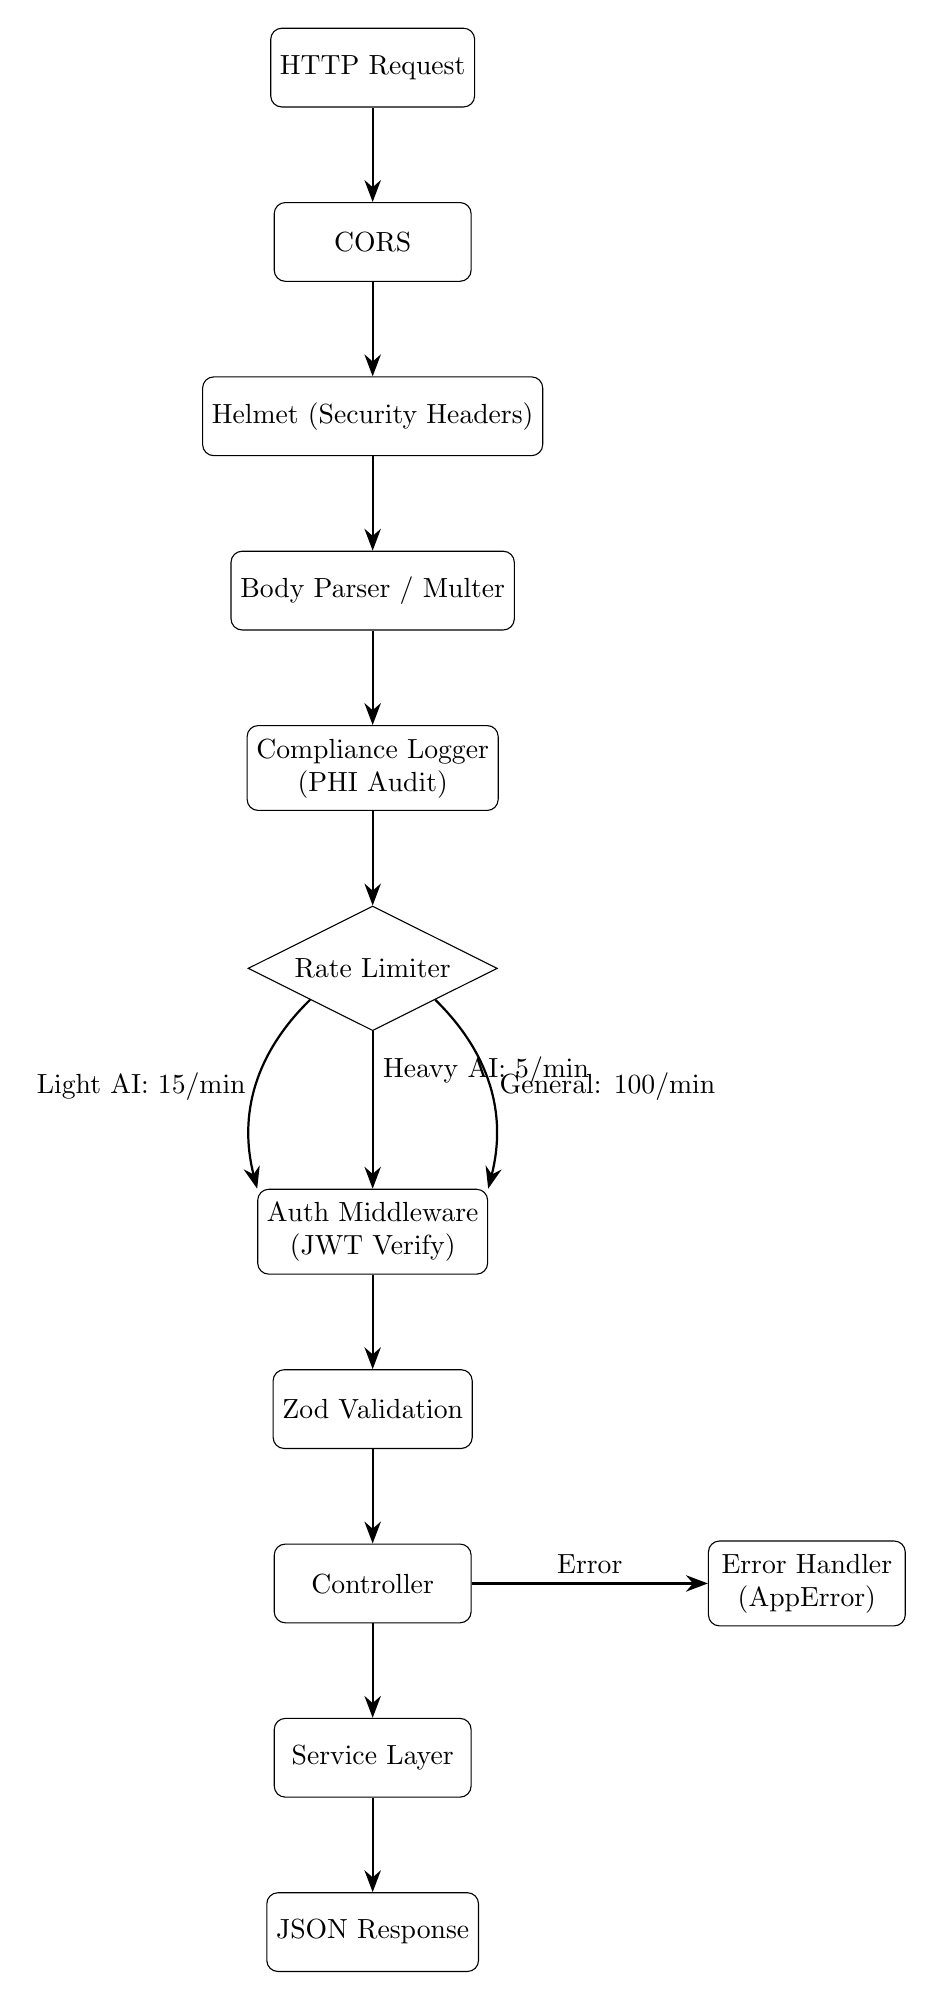
\begin{tikzpicture}[node distance=1.2cm]
    \node[box] (REQ) {HTTP Request};
    \node[box, below=of REQ] (CORS) {CORS};
    \node[box, below=of CORS] (HELMET) {Helmet (Security Headers)};
    \node[box, below=of HELMET] (BODY) {Body Parser / Multer};
    \node[box, below=of BODY] (COMP) {\makecell{Compliance Logger\\(PHI Audit)}};
    \node[diamondbox, below=of COMP] (RL) {Rate Limiter};
    
    \node[box, below=2cm of RL] (AUTH) {\makecell{Auth Middleware\\(JWT Verify)}};
    
    \node[box, below=of AUTH] (VAL) {Zod Validation};
    \node[box, below=of VAL] (CTRL) {Controller};
    \node[box, below=of CTRL] (SVC) {Service Layer};
    \node[box, below=of SVC] (RES) {JSON Response};
    
    \node[box, right=3cm of CTRL] (ERR) {\makecell{Error Handler\\(AppError)}};

    \draw[arrow] (REQ) -- (CORS);
    \draw[arrow] (CORS) -- (HELMET);
    \draw[arrow] (HELMET) -- (BODY);
    \draw[arrow] (BODY) -- (COMP);
    \draw[arrow] (COMP) -- (RL);
    
    \draw[arrow] (RL.south) -- node[right, near start] {Heavy AI: 5/min} (AUTH.north);
    \draw[arrow] (RL.south west) to[bend right=30] node[left] {Light AI: 15/min} (AUTH.north west);
    \draw[arrow] (RL.south east) to[bend left=30] node[right] {General: 100/min} (AUTH.north east);

    \draw[arrow] (AUTH) -- (VAL);
    \draw[arrow] (VAL) -- (CTRL);
    \draw[arrow] (CTRL) -- (SVC);
    \draw[arrow] (SVC) -- (RES);
    \draw[arrow] (CTRL) -- node[above] {Error} (ERR);
\end{tikzpicture}%
}
\end{center}

\newpage
\section*{4. Audio Transcription + Diarization Pipeline}
\resizebox{\textwidth}{!}{%
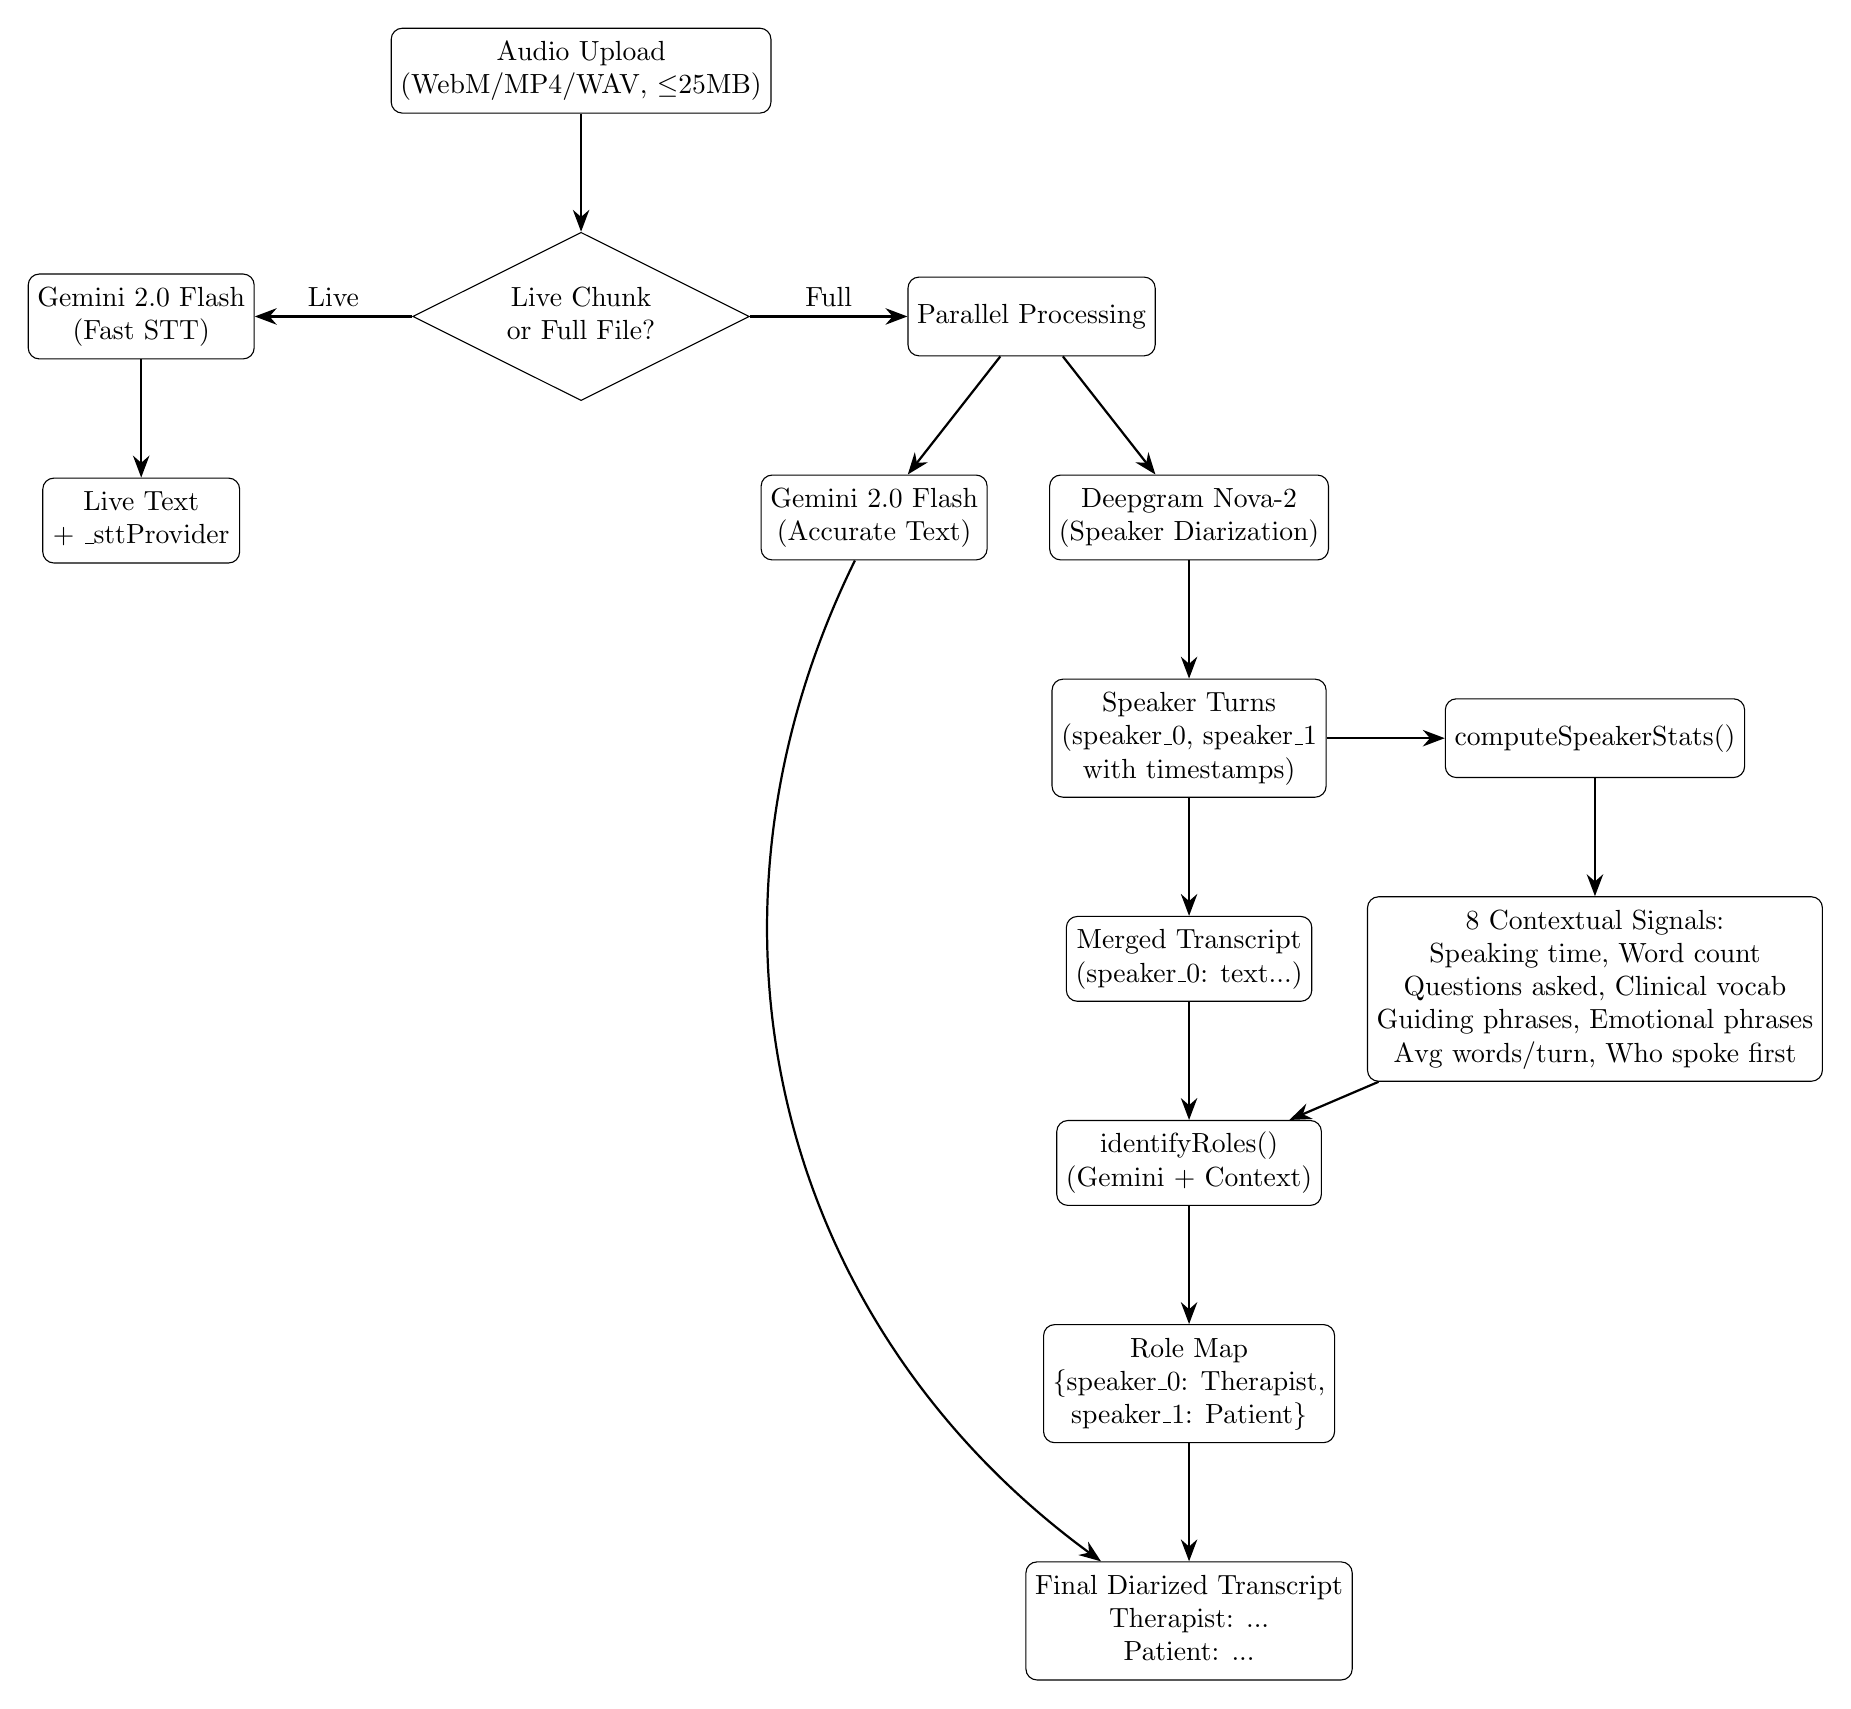
\begin{tikzpicture}[node distance=1.5cm]
    \node[box] (AUDIO) {\makecell{Audio Upload\\(WebM/MP4/WAV, $\le$25MB)}};
    \node[diamondbox, below=of AUDIO] (SPLIT) {\makecell{Live Chunk\\or Full File?}};
    
    \node[box, left=2cm of SPLIT] (GLIVE) {\makecell{Gemini 2.0 Flash\\(Fast STT)}};
    \node[box, below=of GLIVE] (LIVEOUT) {\makecell{Live Text\\+ \_sttProvider}};
    
    \node[box, right=2cm of SPLIT] (PAR) {Parallel Processing};
    \node[box, below=of PAR, xshift=-2cm] (GSTT) {\makecell{Gemini 2.0 Flash\\(Accurate Text)}};
    \node[box, below=of PAR, xshift=2cm] (DEEP) {\makecell{Deepgram Nova-2\\(Speaker Diarization)}};
    
    \node[box, below=of DEEP] (TURNS) {\makecell{Speaker Turns\\(speaker\_0, speaker\_1\\with timestamps)}};
    \node[box, right=of TURNS] (STATS) {computeSpeakerStats()};
    \node[box, below=of STATS] (SIGNALS) {\makecell{8 Contextual Signals:\\Speaking time, Word count\\Questions asked, Clinical vocab\\Guiding phrases, Emotional phrases\\Avg words/turn, Who spoke first}};
    
    \node[box, below=1.5cm of TURNS] (MERGE) {\makecell{Merged Transcript\\(speaker\_0: text...)}};
    \node[box, below=of MERGE] (ROLEID) {\makecell{identifyRoles()\\(Gemini + Context)}};
    \node[box, below=of ROLEID] (ROLES) {\makecell{Role Map\\\{speaker\_0: Therapist,\\speaker\_1: Patient\}}};
    \node[box, below=of ROLES] (FINAL) {\makecell{Final Diarized Transcript\\Therapist: ...\\Patient: ...}};

    \draw[arrow] (AUDIO) -- (SPLIT);
    \draw[arrow] (SPLIT) -- node[above] {Live} (GLIVE);
    \draw[arrow] (GLIVE) -- (LIVEOUT);
    
    \draw[arrow] (SPLIT) -- node[above] {Full} (PAR);
    \draw[arrow] (PAR) -- (GSTT);
    \draw[arrow] (PAR) -- (DEEP);
    \draw[arrow] (DEEP) -- (TURNS);
    \draw[arrow] (TURNS) -- (STATS);
    \draw[arrow] (STATS) -- (SIGNALS);
    \draw[arrow] (TURNS) -- (MERGE);
    \draw[arrow] (MERGE) -- (ROLEID);
    \draw[arrow] (SIGNALS) -- (ROLEID);
    \draw[arrow] (ROLEID) -- (ROLES);
    \draw[arrow] (ROLES) -- (FINAL);
    \draw[arrow] (GSTT) to[bend right=40] (FINAL);
\end{tikzpicture}%
}
\end{center}

\newpage
\section*{5. Database Schema (ERD)}
\resizebox{\textwidth}{!}{%
\begin{tikzpicture}[node distance=3cm]

    \node[box, fill=gray!10, text width=4cm, align=left] (AUTH) {
        \textbf{AUTH\_USERS}\\
        \hline
        PK id (uuid)\\
        email (text)\\
        created\_at (timestamptz)
    };
    
    \node[box, fill=gray!10, text width=4cm, align=left, right=of AUTH] (PAT) {
        \textbf{PATIENTS}\\
        \hline
        PK id (uuid)\\
        FK user\_id (uuid)\\
        name (text)\\
        age (int)\\
        gender (text)\\
        ...\\
        entity\_type (text)
    };

    \node[box, fill=gray!10, text width=4cm, align=left, below=of AUTH] (SESS) {
        \textbf{SESSIONS}\\
        \hline
        PK id (uuid)\\
        FK user\_id (uuid)\\
        FK patient\_id (uuid)\\
        transcript (text)\\
        summary (text)\\
        analysis\_json (jsonb)\\
        audio\_url (text)\\
        session\_mode (text)
    };
    
    \node[box, fill=gray!10, text width=4cm, align=left, right=of SESS] (STOR) {
        \textbf{AUDIO\_STORAGE}\\
        \hline
        path (text)\\
        content\_type (text)\\
        bucket (text)
    };

    \draw[arrow] (AUTH) -- node[above] {owns (1:N)} (PAT);
    \draw[arrow] (AUTH) -- node[left] {records (1:N)} (SESS);
    \draw[arrow] (PAT) -- node[right] {has (1:N)} (SESS);
    \draw[arrow] (SESS) -- node[above] {links to (1:1)} (STOR);

\end{tikzpicture}%
}
\end{center}

\newpage
\section*{6. Summarization \& Analysis Pipeline}
\resizebox{\textwidth}{!}{%
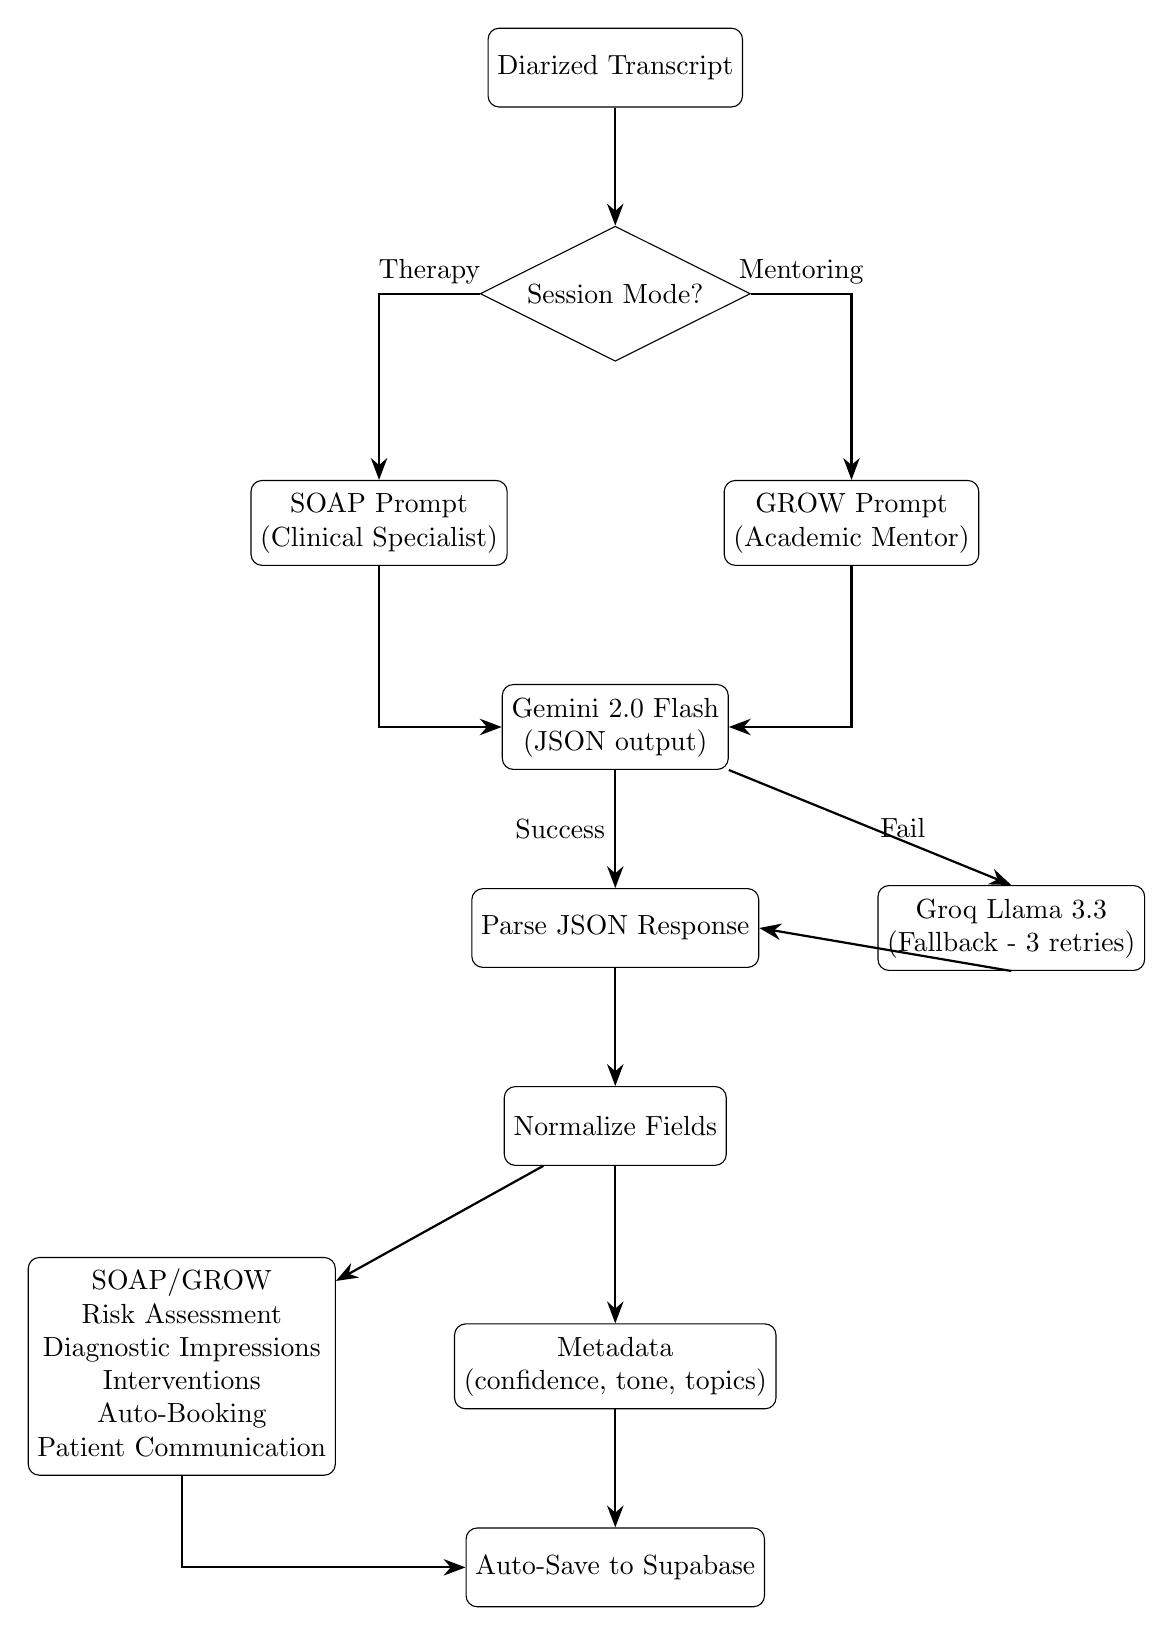
\begin{tikzpicture}[node distance=1.5cm]
    \node[box] (TRANS) {Diarized Transcript};
    \node[diamondbox, below=of TRANS] (MODE) {Session Mode?};
    
    \node[box, below=of MODE, xshift=-3cm] (SOAP) {\makecell{SOAP Prompt\\(Clinical Specialist)}};
    \node[box, below=of MODE, xshift=3cm] (GROW) {\makecell{GROW Prompt\\(Academic Mentor)}};
    
    \node[box, below=of SOAP, xshift=3cm] (GEMINI) {\makecell{Gemini 2.0 Flash\\(JSON output)}};
    
    \node[box, below=of GEMINI] (PARSE) {Parse JSON Response};
    \node[box, right=of PARSE] (GROQ) {\makecell{Groq Llama 3.3\\(Fallback - 3 retries)}};
    
    \node[box, below=of PARSE] (NORM) {Normalize Fields};
    
    \node[box, below=2cm of NORM] (META) {\makecell{Metadata\\(confidence, tone, topics)}};
    \node[box, left=of META] (OUTPUT) {\makecell{SOAP/GROW\\Risk Assessment\\Diagnostic Impressions\\Interventions\\Auto-Booking\\Patient Communication}};
    
    \node[box, below=of META] (SAVE) {Auto-Save to Supabase};

    \draw[arrow] (TRANS) -- (MODE);
    \draw[arrow] (MODE) -| node[above, near start] {Therapy} (SOAP);
    \draw[arrow] (MODE) -| node[above, near start] {Mentoring} (GROW);
    \draw[arrow] (SOAP) |- (GEMINI);
    \draw[arrow] (GROW) |- (GEMINI);
    
    \draw[arrow] (GEMINI) -- node[left] {Success} (PARSE);
    \draw[arrow] (GEMINI.south east) -- node[right] {Fail} (GROQ.north);
    \draw[arrow] (GROQ.south) -- (PARSE.east);
    
    \draw[arrow] (PARSE) -- (NORM);
    \draw[arrow] (NORM) -- (OUTPUT);
    \draw[arrow] (NORM) -- (META);
    \draw[arrow] (OUTPUT) |- (SAVE);
    \draw[arrow] (META) -- (SAVE);

\end{tikzpicture}%
}
\end{center}

\newpage
\section*{7. Security \& Access Control Layers}
\resizebox{\textwidth}{!}{%
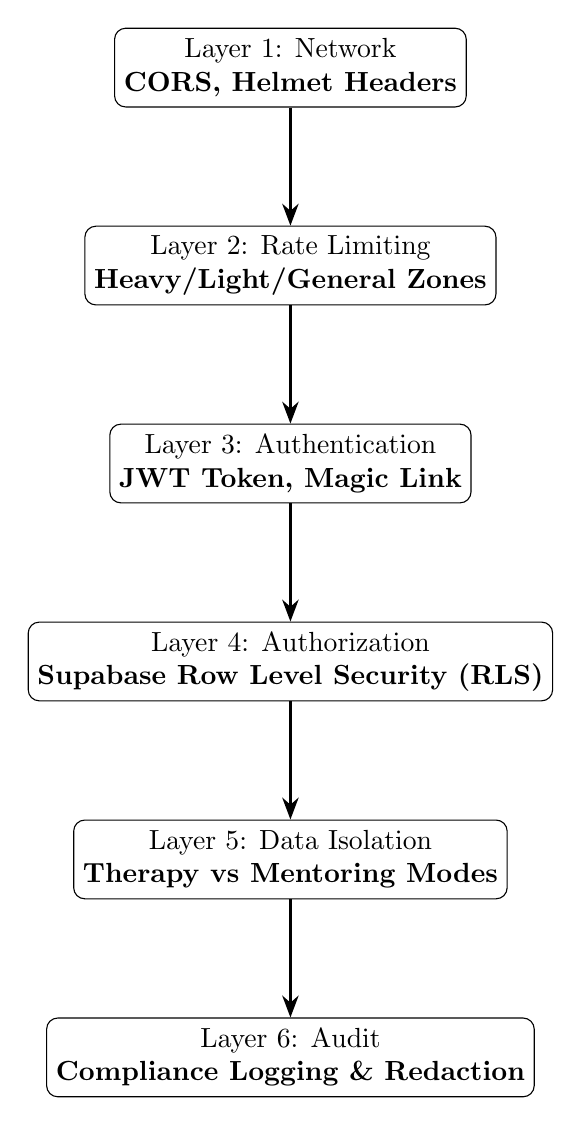
\begin{tikzpicture}[node distance=1.5cm]
    \node[box] (L1) {Layer 1: Network \\ \textbf{CORS, Helmet Headers}};
    \node[box, below=of L1] (L2) {Layer 2: Rate Limiting \\ \textbf{Heavy/Light/General Zones}};
    \node[box, below=of L2] (L3) {Layer 3: Authentication \\ \textbf{JWT Token, Magic Link}};
    \node[box, below=of L3] (L4) {Layer 4: Authorization \\ \textbf{Supabase Row Level Security (RLS)}};
    \node[box, below=of L4] (L5) {Layer 5: Data Isolation \\ \textbf{Therapy vs Mentoring Modes}};
    \node[box, below=of L5] (L6) {Layer 6: Audit \\ \textbf{Compliance Logging \& Redaction}};
    
    \draw[arrow] (L1) -- (L2);
    \draw[arrow] (L2) -- (L3);
    \draw[arrow] (L3) -- (L4);
    \draw[arrow] (L4) -- (L5);
    \draw[arrow] (L5) -- (L6);
\end{tikzpicture}%
}
\end{center}

\newpage
\section*{8. Export \& Communication Flow}
\resizebox{\textwidth}{!}{%
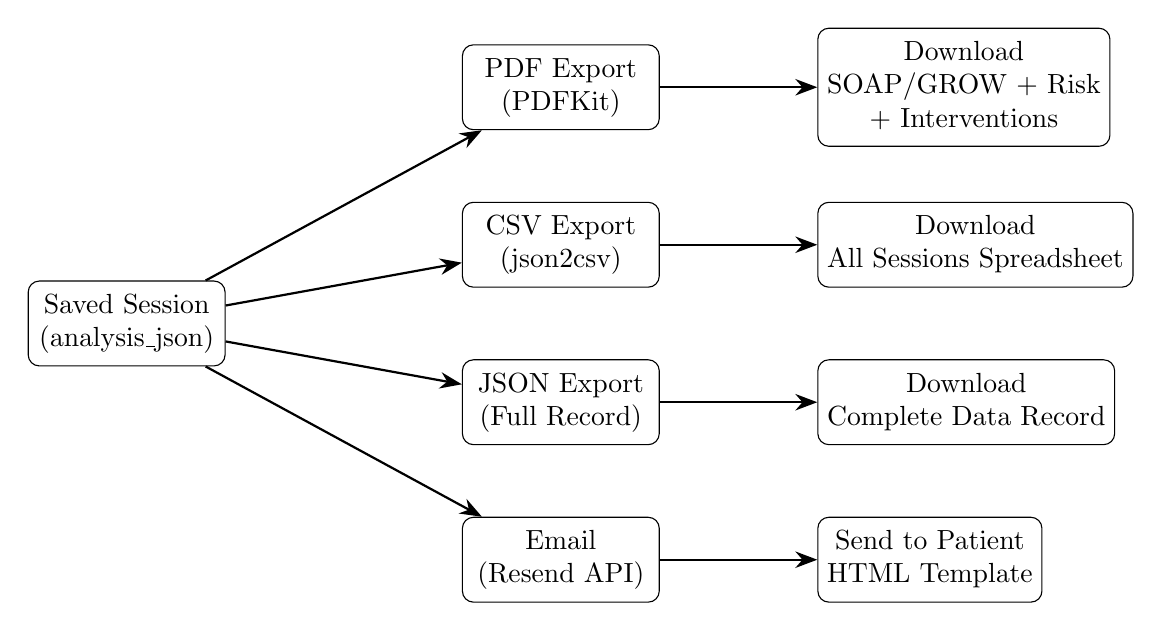
\begin{tikzpicture}[node distance=1.5cm and 2cm]
    \node[box] (SESS) {\makecell{Saved Session\\(analysis\_json)}};
    
    \node[box, right=3cm of SESS, yshift=3cm] (PDF) {\makecell{PDF Export\\(PDFKit)}};
    \node[box, right=3cm of SESS, yshift=1cm] (CSV) {\makecell{CSV Export\\(json2csv)}};
    \node[box, right=3cm of SESS, yshift=-1cm] (JSON) {\makecell{JSON Export\\(Full Record)}};
    \node[box, right=3cm of SESS, yshift=-3cm] (EMAIL) {\makecell{Email\\(Resend API)}};
    
    \node[box, right=of PDF] (DL_PDF) {\makecell{Download\\SOAP/GROW + Risk\\+ Interventions}};
    \node[box, right=of CSV] (DL_CSV) {\makecell{Download\\All Sessions Spreadsheet}};
    \node[box, right=of JSON] (DL_JSON) {\makecell{Download\\Complete Data Record}};
    \node[box, right=of EMAIL] (DL_EMAIL) {\makecell{Send to Patient\\HTML Template}};
    
    \draw[arrow] (SESS) -- (PDF);
    \draw[arrow] (SESS) -- (CSV);
    \draw[arrow] (SESS) -- (JSON);
    \draw[arrow] (SESS) -- (EMAIL);
    
    \draw[arrow] (PDF) -- (DL_PDF);
    \draw[arrow] (CSV) -- (DL_CSV);
    \draw[arrow] (JSON) -- (DL_JSON);
    \draw[arrow] (EMAIL) -- (DL_EMAIL);
\end{tikzpicture}%
}
\end{center}

\newpage
\section*{9. Proposed Work Plan}
\begin{center}
\resizebox{\textwidth}{!}{%
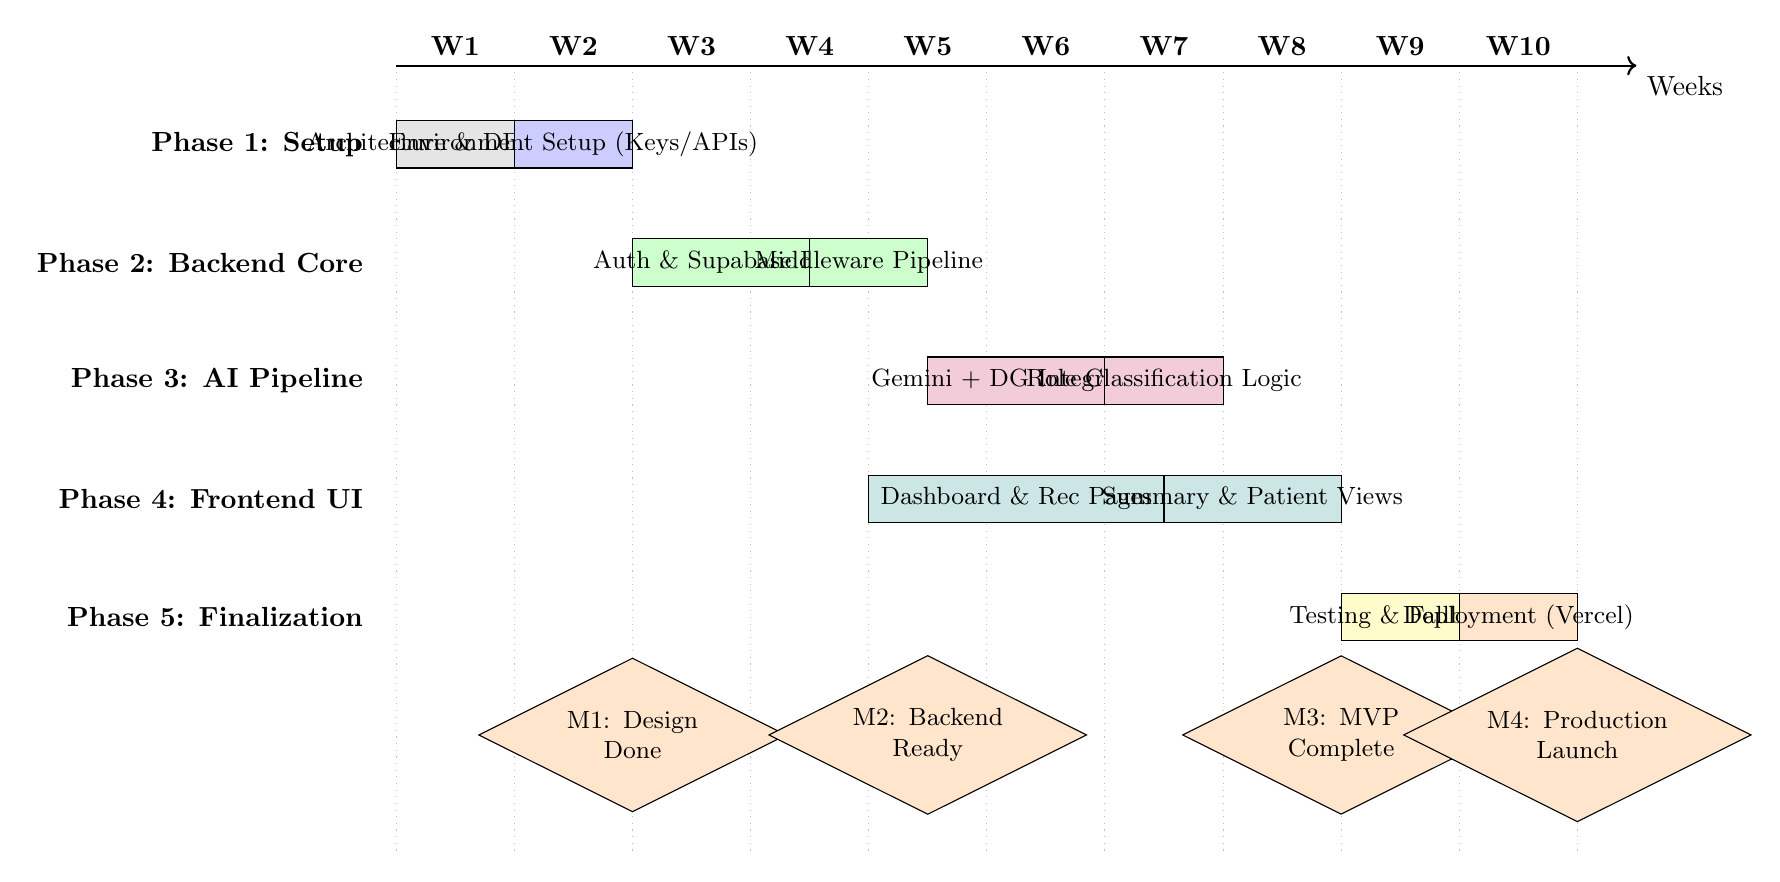
\begin{tikzpicture}[
    x=1.5cm, y=-1cm,
    task/.style={draw, rectangle, rounded corners=2pt, minimum height=0.6cm, align=left, fill=blue!10, text width=4cm, font=\small},
    milestone/.style={draw, diamond, aspect=2, minimum height=0.6cm, align=center, fill=orange!20, font=\small},
    grid/.style={dotted, gray!50}
]

    % Header row (Weeks)
    \foreach \w in {1,...,10} {
        \node[anchor=south] at (\w-0.5, 0) {\textbf{W\w}};
        \draw[grid] (\w, 0) -- (\w, 10);
    }
    \draw[grid] (0, 0) -- (0, 10);

    % Phase 1: Planning & Setup
    \node[anchor=east, font=\bfseries] at (-0.2, 1) {Phase 1: Setup};
    \draw[fill=gray!20] (0, 0.7) rectangle node[font=\small] {Architecture \& DB Design} (1, 1.3);
    \draw[fill=blue!20] (1, 0.7) rectangle node[font=\small] {Environment Setup (Keys/APIs)} (2, 1.3);

    % Phase 2: Core Backend Core
    \node[anchor=east, font=\bfseries] at (-0.2, 2.5) {Phase 2: Backend Core};
    \draw[fill=green!20] (2, 2.2) rectangle node[font=\small] {Auth \& Supabase RLS} (3.5, 2.8);
    \draw[fill=green!20] (3.5, 2.2) rectangle node[font=\small] {Middleware Pipeline} (4.5, 2.8);
    
    % Phase 3: AI Pipeline
    \node[anchor=east, font=\bfseries] at (-0.2, 4) {Phase 3: AI Pipeline};
    \draw[fill=purple!20] (4.5, 3.7) rectangle node[font=\small] {Gemini + DG Integration} (6, 4.3);
    \draw[fill=purple!20] (6, 3.7) rectangle node[font=\small] {Role Classification Logic} (7, 4.3);
    
    % Phase 4: Frontend MVP
    \node[anchor=east, font=\bfseries] at (-0.2, 5.5) {Phase 4: Frontend UI};
    \draw[fill=teal!20] (4, 5.2) rectangle node[font=\small] {Dashboard \& Rec Pages} (6.5, 5.8);
    \draw[fill=teal!20] (6.5, 5.2) rectangle node[font=\small] {Summary \& Patient Views} (8, 5.8);

    % Phase 5: Polish & Security
    \node[anchor=east, font=\bfseries] at (-0.2, 7) {Phase 5: Finalization};
    \draw[fill=yellow!20] (8, 6.7) rectangle node[font=\small] {Testing \& Fallbacks} (9, 7.3);
    \draw[fill=orange!20] (9, 6.7) rectangle node[font=\small] {Deployment (Vercel)} (10, 7.3);

    % Milestones
    \node[milestone, text width=2cm] at (2, 8.5) {M1: Design\\Done};
    \node[milestone, text width=2cm] at (4.5, 8.5) {M2: Backend\\Ready};
    \node[milestone, text width=2cm] at (8, 8.5) {M3: MVP\\Complete};
    \node[milestone, text width=2.5cm] at (10, 8.5) {M4: Production\\Launch};
    
    % Labels axis
    \draw[thick, ->] (0, 0) -- (10.5, 0) node[anchor=north west] {Weeks};

\end{tikzpicture}%
}
\end{center}

\end{document}
